%============================================================================
% tento soubor pouzijte jako zaklad
% (c) 2008 Michal Bidlo
% E-mail: bidlom AT fit vutbr cz
%============================================================================
% kodovaní: iso-8859-2 (zmena prikazem iconv, recode nebo cstocs)
%----------------------------------------------------------------------------
% zpracování: make, make pdf, make desky, make clean
% připomínky posílejte na e-mail: bidlom AT fit.vutbr.cz
% vim: set syntax=tex encoding=latin2:
%============================================================================
\documentclass[cover, english]{fitthesis} % odevzdani do wisu - odkazy, na ktere se da klikat
%\documentclass[cover,print]{fitthesis} % pro tisk - na odkazy se neda klikat
%\documentclass[english,print]{fitthesis} % pro tisk - na odkazy se neda klikat
%      \documentclass[english]{fitthesis}
% * Je-li prace psana v anglickem jazyce, je zapotrebi u tridy pouzit 
%   parametr english nasledovne:
%      \documentclass[english]{fitthesis}
% * Neprejete-li si vysazet na prvni strane dokumentu desky, zruste 
%   parametr cover

% zde zvolime kodovani, ve kterem je napsan text prace
% "latin2" pro iso8859-2 nebo "cp1250" pro windows-1250, "utf8" pro "utf-8"
%\usepackage{ucs}
\usepackage[utf8]{inputenc}
\usepackage[T1, IL2]{fontenc}
\usepackage{url}
\DeclareUrlCommand\url{\def\UrlLeft{<}\def\UrlRight{>} \urlstyle{tt}}

%zde muzeme vlozit vlastni balicky
\usepackage{todonotes}
\usepackage{listings}

% =======================================================================
% balíček "hyperref" vytváří klikací odkazy v pdf, pokud tedy použijeme pdflatex
% problém je, že balíček hyperref musí být uveden jako poslední, takže nemůže
% být v šabloně
\ifWis
\ifx\pdfoutput\undefined % nejedeme pod pdflatexem
\else
  \usepackage{color}
  \usepackage[unicode,colorlinks,hyperindex,plainpages=false,pdftex]{hyperref}
  \definecolor{links}{rgb}{0.4,0.5,0}
  \definecolor{anchors}{rgb}{1,0,0}
  \def\AnchorColor{anchors}
  \def\LinkColor{links}
  \def\pdfBorderAttrs{/Border [0 0 0] }  % bez okrajů kolem odkazů
  \pdfcompresslevel=9
\fi
\fi

%Informace o praci/projektu
%---------------------------------------------------------------------------
\projectinfo{
  %Prace
  project=DP,            %typ prace BP/SP/DP/DR
  year=2015,             %rok
  date=\today,           %datum odevzdani
  %Nazev prace
  title.cs={Portace nástroje OptaPlanner na Android},  %nazev prace v cestine
  title.en={Port of OptaPlanner on Android}, %nazev prace v anglictine
  %Autor
  author={Tomáš David},   %jmeno prijmeni autora
  %author.title.p=Bc., %titul pred jmenem (nepovinne)
  %author.title.a=PhD, %titul za jmenem (nepovinne)
  %Ustav
  department=UITS, % doplnte prislusnou zkratku: UPSY/UIFS/UITS/UPGM
  %Skolitel
  supervisor=Zdeněk Letko, %jmeno prijmeni skolitele
  supervisor.title.p=Ing.,   %titul pred jmenem (nepovinne)
  supervisor.title.a={Ph.D.},    %titul za jmenem (nepovinne)
  %Klicova slova, abstrakty, prohlaseni a podekovani je mozne definovat 
  %bud pomoci nasledujicich parametru nebo pomoci vyhrazenych maker (viz dale)
  %===========================================================================
  %Klicova slova
  keywords.cs={OptaPlanner, Android, portace}, %klicova slova v ceskem jazyce
  keywords.en={OptaPlanner, Android, portation}, %klicova slova v anglickem jazyce
  %Abstract
  abstract.cs={Tato práce se zabývá nástrojem OptaPlanner, který se využívá pro řešení plánovacích problému. Dále je v práci popsána platforma Android -- operační systém určený pro mobilní zařízení. V poslední řadě ze zabývá portací nástroje OptaPlanner na tuto platformu.}, % abstrakt v ceskem jazyce
  abstract.en={This thesis deals with OptaPlanner tool, which is used for solving optimization problems. This work describes Android platform -- an operating system for mobile devices. Finally, it deals with port of OptaPlanner on this platform.}, % abstrakt v anglickem jazyce
  %Prohlaseni
  declaration={Prohlašuji, že jsem tuto diplomovou práci vypracoval samostatně pod vedením pana Ing. Zdeňka Letka, Ph.D.},
  %Podekovani (nepovinne)
  acknowledgment={Rád bych poděkoval mému vedoucímu Ing. Zdeňku Letkovi, Ph.D. a mému konzultantovi Geoffrey De Smetovi za cenné rady a věcné připomínky při řešení projektu.} % nepovinne
}

%Abstrakt (cesky, anglicky)
%\abstract[cs]{Do tohoto odstavce bude zapsán výtah (abstrakt) práce v českém jazyce.}
%\abstract[en]{Do tohoto odstavce bude zapsán výtah (abstrakt) práce v anglickém jazyce.}

%Klicova slova (cesky, anglicky)
%\keywords[cs]{Sem budou zapsána jednotlivá klíčová slova v českém jazyce, oddělená čárkami.}
%\keywords[en]{Sem budou zapsána jednotlivá klíčová slova v anglickém jazyce, oddělená čárkami.}

%Prohlaseni
%\declaration{Prohlašuji, že jsem tuto bakalářskou práci vypracoval samostatně pod vedením pana X...
%Další informace mi poskytli...
%Uvedl jsem všechny literární prameny a publikace, ze kterých jsem čerpal.}

%Podekovani (nepovinne)
%\acknowledgment{V této sekci je možno uvést poděkování vedoucímu práce a těm, kteří poskytli odbornou pomoc
%(externí zadavatel, konzultant, apod.).}

\begin{document}
  % Vysazeni titulnich stran
  % ----------------------------------------------
  \maketitle
  % Obsah
  % ----------------------------------------------
  \tableofcontents
  
  % Seznam obrazku a tabulek (pokud prace obsahuje velke mnozstvi obrazku, tak se to hodi)
  % \listoffigures
  % \listoftables 

  % Text prace
  % ----------------------------------------------
  %\chapter{Úvod}
\chapter{Introduction}
Porting of applications becomes very actual issue in the modern world of information technology. Every operating system uses own interface and technologies for application development. However, there are tools that are cross-platform allowing of porting the applications without much interference. One of these tools is the Java programming language.

Java languge is developed by Oracle Corporation and it is distributed in several platforms. The most common platform is Java Standart Edition which contains many of the basic Java libraries which are ordinarily used in standart desktop applications. A set of these libraries is is called the Java SE API.

Android is and operating system for mobile devices developed by Google. It uses the Java programming language to application development. Android runtime environment includes not only the libraries for development of user interface of Android applications but also subset of Java SE API libraries.

OptaPlanner is an open source software developed by JBoss community designed for solving planning problems. It is completely writen in Java and its easy portable between desktop opetaing system. However, Android API does not contains all of the Java SE API libraries and therefore porting of the OptaPlanner tool may cause problems with dependencies.

This term project is divided into six chapters. Chapter~\ref{JavaChapter} presents the Java programing language and its platforms. Chapter~\ref{AndroidChapter} describes the Android platform, its architecture and the build process. Chapter~\ref{OptaPlannerChapter} explains what the OptaPlanner tool is and shows its configuration. In the Chapter~\ref{PortingChapter}, differences between Java SE API and Android API are described and the possible solutions of the JavaBeans problem on the Android platform are suggested. The last Chapter~\ref{ConclusionChapter} summarizes the entire work.



%\chapter{Teorie}
\chapter{Theory}
\section{Java}
Java je jedním z nejpoužívanějších a nejpopulárnějších počítačových programovacích jazyků na světě. Syntaxe tohoto jazyka se řadí k těm jednodužším, avšak jeho použití je velmi rozsáhlé. V Java se programují čipové karty, mobilní a desktopové aplikace, i velké podnikové a informační systémy. Java je jazyk multiplatformní a díky tomu je jej možné použít ná různých operačních systémech. Java je vyvíjena jako OpenSource. Java se objevuje ve třech základních edicích:


\subsection{Java platformy}
Jazyk Java je společně s virtuálním strojem a knihovnami vydáván ve čtyřech platformách, kde každá má své speciální určení.

\subsubsection{Java SE}
Základní platforma pro vývoj desktopových a jednodužších serverových aplikací. V součané době je poslední vydaná verze Java SE 8u25.

\subsubsection{Java EE}
Nádstavba nad Java SE obsahující speciální knihovny pro vývoj a provoz podnikových aplikací a informačních systémů. V součané době je poslední vydaná verze Java EE 7.

\subsubsection{Java ME (Micro Edition)}
Podmnožina Java SE pro vývoj aplikací pro malá zařízení jako jsou mikrokontroléry sensory, mobilní telefony, set-top boxy, tiskárny a další. V součané době je poslední vydaná verze Java ME 8.1.

\subsubsection{Java Card}
Verze určená pro vývoj aplikací určených pro čipové karty a pro zařízení s limitovanou pamětí a schopností zpracovávání. Příkladem mohou být SIM karty pro mobilní zařízení nebo čipové karty pro ATM bankomaty. V součané době je poslední vydaná verze Java Card 3.0.4.

\subsection{Vývojářské sady}
Možnosti jak Javu stáhnout jsou dvě. Jedná se o balík se kterým lze pouze spouštět aplikace Java (JRE) nebo balík který slouží pro vývoj (JDK).

\subsubsection{Java JRE (Java Runtime Environment)}
Běhové prostředí Javy, které poskytuje vše potřebné pro suštění java aplikací. Součástí je virtuální stroj javy a potřebné knihovny.

\subsubsection{Java JDK (Java Development Kit)}
Někdy se také označuje SDK (Software Development Kit). Jedná se o sadu JRE doplněnou o vyvojářské nástroje (překladač, generátor dokumentace, ladící nástroje a další).

\begin{figure}[h!]
    \centering
    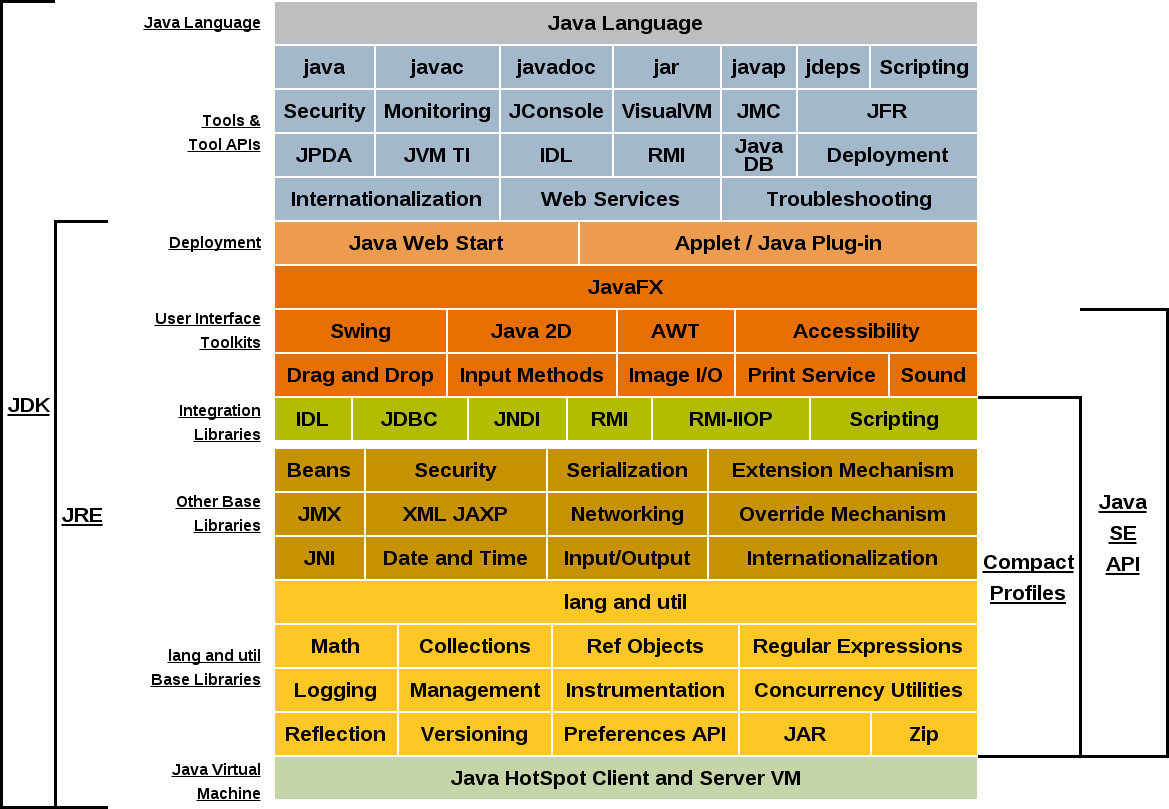
\includegraphics[scale=0.3]{fig/java_jdk.jpg}
    \caption{Java SE JDK 1.8}
\end{figure}



\section{Android}



\section{Gradle}


\section{JBoss Drools}

  \subsection{Drools Expert}

  \subsection{OptaPlanner}


\section{Vehicle routing problem}

%\subsection{History}
%V následující tabulce je stručně popsána historie programovacího jazyku Java: \\
%\\
%\begin {table}[h!]
%\begin{tabular}{|l|l|l|}[h]
%\hline
%    {\bf Název} & {\bf Datum} & {\bf Poznámka}  \\
%    \hline \hline
%    Oak         & 1991                  & a     \\
%    JDK         & 1995                  & a     \\
%    JDK 1.0     & January 23rd, 1996    & a     \\
%    JDK 1.1     & February 19th, 1997   & a     \\
%    JPE         & May, 1998             & a \\
%    J2SE 1.2    & December 8th, 1998    & a     \\
%    J2EE 1.2    & December 12, 1999     & a     \\
%    J2SE 1.3    & May 8th, 2000         & a     \\
%    J2EE 1.3    & September 24, 2001    & a \\
%    J2SE 1.4    & February 6th, 2002    & a     \\
%    J2EE 1.4    & November 11, 2003     & a \\
%    J2SE 5.0    & September 30th, 2004  & a     \\
%    Java EE 5   & May 11, 2006          & a \\
%    Java SE 6   & December 11th, 2006   & a     \\
%    Java EE 6   & December 10, 2009     & a \\
%    Java SE 7   & July 28th, 2011       & a     \\
%    Java EE 7   & June 12, 2013         & a \\
%    Java SE 8   & March 18th, 2014      & a     \\
%  \hline
%\end{tabular}
%\caption{Historie Javy}
%\end{table}






%\chapter{Portace}
\chapter{Port}
tady popsat rozdil java jdk a android api
java beans problem
problemy android aplikaci


\section{Java SE API and Android API}
Android API je postaveno na Java SE 6, avšak jak je možno vidět na tabulce \todo{odkaz na tabulku} není kompletní Java SE API. Podstatná část balíčků chybí nebo jsou některé ne zcela kompletní. V případě balíčku uživatelského rozhraní jako je java.awt a java swing byly nahrazeny androidími grafickými uživatelskými prvky. Některé balíčky však nemusejí mít přímou souvislost s grafickým uživatelským rozhraním, a proto při portování aplikací můžeme narazit na problém s jejich nedispozicí.

\begin {table}[h!]
\begin{tabular}{|l|l|}
\hline
{\bf Java 6 SE Package} & {\bf Included in Android API} \\
\hline \hline
java.applet             & No -- missing completely    \\
java.awt                & Yes -- incomplete            \\
java.beans              & Yes -- incomplete            \\
java.io	                & Yes -- complete            \\
java.lang	            & Yes -- incomplete            \\
java.math	            & Yes -- complete            \\
java.net	            & Yes -- complete             \\
java.nio	            & Yes -- complete             \\
java.rmi	            & No  -- missing completely    \\
java.security	        & Yes -- incomplete            \\
java.sql	            & Yes -- complete            \\
java.text	            & Yes -- complete              \\
java.util	            & Yes -- incomplete            \\
javax.accessibility     & No -- missing completely    \\
javax.activation	    & No -- missing completely    \\
javax.activity	        & No -- missing completely    \\
javax.annotation	    & No -- missing completely    \\
javax.crypto	        & Yes -- complete              \\
javax.imageio	        & No -- missing completely    \\
javax.jws	            & No -- missing completely    \\
javax.lang	            & No -- missing completely    \\
javax.management        & No -- missing completely    \\
javax.naming	        & No -- missing completely    \\
javax.net	            & Yes -- complete              \\
javax.print		        & No -- missing completely    \\
javax.rmi		        & No -- missing completely    \\
javax.script	        & No -- missing completely    \\
javax.security          & Yes -- incomplete            \\
javax.sound             & No -- missing completely    \\
javax.sql	            & Yes -- incomplete javax.sql  \\
javax.swing	            & No -- missing completely    \\
javax.tools	            & No -- missing completely    \\
javax.transaction	    & No -- missing completely    \\
javax.xml	            & Yes -- incomplete            \\
org.ietf.jgss	        & No -- missing completely    \\
org.omg                 & No -- missing completely    \\
org.w3c.dom             & Yes -- incomplete            \\
org.xml.sax	            & Yes -- complete              \\
\hline
\end{tabular}
\centering
\caption{Java 6 SE packages in Android API}
\end{table}

\section{JavaBeans}
OptaPlanner je kompletně napsán v programovacím jazyce Java a jednou z jeho závislostí jsou třídy z balíčeku java.beans. Jak je možno vidět v tabulce tento balíček je nekompletní. Při spuštění jednoduchého OptaPlanner projektu vznikne vyjímka ClassNotFoundException, právě z důvodu, že potřebné třídy se v tomto balíčku nenacházejí.   V této sekci si ukážeme jak tento jaké jsou možnosti řešení tohoto problému.

\subsection{Přebalení Java Beans redistribuce do java namespace}
Prvním ze způsobů jak nahradit chybějící balík java.beans je využití redistribuce JavaBeans. Jedná se knihovny speciálně určené pro Android platformu pro podporu JavaBeans či dalších knihoven. Tyto knihovny je potřeba přebalit pomocí nástroje JarJar Links do namespace java.beans a výsledný jar soubor přiložit k android projektu. 

\subsubsection{OpenBeans}
OpenBeans jsou redistribuce java.beans balíčku z Apache Harmony projektu. Namespace se ale od java.beans balíšku líší, v openbeans se používá com.googlecode.openbeans namespace. Vznikly v prvé řadě právě díky neexistenci java.beans na platformě Android. Jedná se o opensource projekt a je distribuován jako jar balíček, který je možné přidat do svého projektu. 

\subsubsection{Mad Robot}
Podobný projekt jako je OpenBeans se nazývá Mad Robot. Stejně jako OpenBeans obsahuje redistribuci balíčku java.beans pod namespace com.madrobot.beans a navíc přidává i některé další balíčky např pro práci s databází, s grafikou, geometrií atd. Tento projekt je distribuován ve formě Maven závislostí.

\subsubsection{Jar Jar Links}
Jar Jar Links je nástroj pro přebalování Java knihoven. Umožňuje za přebalit java třídy z jednoho namespace do druhého. Proces probíhá pomocí pomocného souboru, kde se určí pravidla a způsob přebalení. Nakonec se pomocí příkazu spustí proces.
\\
\begin{lstlisting}[captionpos={b},caption={Spanning tree broadcast algorithm.},frame={lines},label={rule},basicstyle=\footnotesize]
rule com.googlecode.openbeans.** java.beans.@1
\end{lstlisting}

\begin{lstlisting}[captionpos={b},caption={Spanning tree broadcast algorithm.},frame={lines},label={command},basicstyle=\footnotesize]
java -jar jarjar.jar process rule.txt openbeans.jar javabeans.jar
\end{lstlisting}

\subsubsection{Core library flag}
Při překladu android aplikace, která obsahuje třídy z namespace java.* nebo javax.* dojde k chybě, která upozorňuje na používání tříd z java core namespace. Tomuto se dá předejít použitím flagu --core-library v nástroji dx, který je umístěn v android-sdk ve složce build tools. Přidáním flagu na poslední řádek povolí překlad aplikace. V listungu je možné vidět jak tento řádek má vypadat.\todo{přidat zmínku k ostatním}
\\
\begin{lstlisting}[captionpos={b},caption={Spanning tree broadcast algorithm.},frame={lines},label={command},basicstyle=\footnotesize]
exec java $javaOpts -jar "$jarpath" --core-library "$@"
\end{lstlisting}

\subsection{Použití zdrojových kódu openJDK distribuce}
Toto řešení zakládá na využití dostupných zdrojových kódu Java SE. Díky tomu je možné získat potřebné knihovny a přidat je přimo do svého projektu. Výhoda tohoto řešení je že se chyby závislostí ukáží už při překladu a ne až když beží aplikace. Díky tomu je možné si ze zdrojových kódu vybrat to potřebné. Tato upráva však není triviální a buď je potřeba použít speciální nástroje které odstraní nepoužívané závislosti nebo postup udělat manuálně. 

\subsection{Použití prořezaného rt.jar}
Poslední možnoistí bez zásahu do zdrojového kódu je použití balíku rt.jar který je součást knihoven Java SE. Tento balík obsahuje zkompilované třídy JavaBeans a další součásti Java SE. Díky své velikosti se však příliš nehodí pro android aplikace a navíc obsahuje i knihovny které Android API obsahuje a proto by docházelo ke kolizím. Proto je nutné jej prořezat. Výhodou tohoto přořezání je že se nemusíme starat o závislosti, které nejsou potřeba pro Optaplanner nástroj, protože tyto soubory již neprocházejí java kompilátorem. Na druhou stranu se může stát že během běhu aplikace se narazí na potřebnou závislost a aplikace vyhodí vyjímku a aplikace spadne.

\subsection{Použití OpenBeans v OptaPlanner projektu}
První možností při které je nutné zasahovat do zdrojového kódu je nahrazení závislostí java.beans za com.googlecode.openbeans. Tímto přepsáním importů a připojením balíčku openbeans.jar do jde k přeměrování na třídy open beans. Névyhodou tohoto řešení je právě zásah do zdrojových kódu optaplanneru. Z hlediska vývojáře android aplikace je potřeba vytvořit nový "fork" optaplanneru a ten upravit. A při nové verzi optaplanneru závést změny. Údržba je pak značně komplikovaná.

\subsection{Odstranění a nahrazení JavaBeans z OptaPlanneru}
Poslední možnost vyřešení problému JavaBeans jeho odstranění ze zdrojového kódu a nahrazení jinou technologií. Nevýhody tohoto řešení zpočívají především v zásahu do zdrojových kódů. V podstatě by se jednalo o největší zásah z nábízených řešení. 

\subsection{Shrnutí jednotlivých přístupů}
V následující tabulce je možné vidět jaké jsou výhody a nevýhody jednotlivých řečení. Dále jsou přidány licence, které je potřeba respektovat při použití:
\begin {table}[h!]
\begin{tabular}{|p{2.5cm}|p{2cm}|p{2.4cm}|p{2.1cm}|p{5cm}|}
\hline
{\bf Přístup} & {\bf Licence} & {\bf Optaplanner modification} & {\bf Complexity} & {\bf Notes} \\
\hline \hline
Použití přebaleného OpenBean redistribuce & Apache License 2.0 & No & Easy & 
{\bf Výhovy:} samostatný soubor jar, bez problémů se závistlostmi \\
\hline
Použití přebaleného Mad Robot redistribuce & LGPL 2.1 & No & Easy &  stejné jako předchozí \\
\hline
Použití zdrojových kódu openJDK distribuce &  GPL 2.0 / proprietary\footnotemark & No & Hard &
+ chyby závislostí se objeví už při překladu
+ kontrola nad zdrojovými kódy
- obtížná úprava
- soubory nejsou v samostatném jar \\
\hline
Použití prořezaného rt.jar & GPL 2.0 / proprietary & No & Hard & 
+ samostatný soubor jar
+ není potřeba řešit závislosti pro spravný překlad
- nutnost prořezání
- obtížnější úprava
- možné problémy se závislostmi
- nekonzistentní jar\\
\hline
Použití OpenBeans v OptaPlanner projektu & Apache License 2.0 & Yes & Easy &
{\bf Výhovy:} Jednoduchá úprava

{\bf Nevýhovy:} nutnost úpravy optaplanner kódu a jeho
následná údržby forku optaplanneru \\
\hline
Odstranění a nahrazení JavaBeans z OptaPlanneru & -- & Yes & Medium &
{\bf Nevýhovy:} stejné jako v předchozím případě \\
\hline
\end{tabular}
\centering
\caption{Java 6 SE packages in Android API}
\end{table}


\footnotetext{This is my footnote!}





%\chapter{Závěr}
\chapter{Conclusion}
Libraries of Java SE API and Android API were compared and it was found that they differ significantly. Out of 38 Java
SE API packages, 20 packages are completely missing and 9 packages are incomplete in Android API. On closer inspection,
it was revealed that one of the OptaPlanner tool dependencies is missing in Android API. This missing package is named
JavaBeans.

For JavaBeans problem were suggested five solutions, namely: Repacking JavaBeans redistribution to Java core namespace,
Use of OpenJDK distribution source code, Use of pruned rt.jar from OpenJDK distribution, Use of OpenBeans in
OptaPlanner project and Removing and replacing JavaBeans from OptaPlanner. Due to comparison of advantages and
disadvantages of individual solutions, it was selected a~solution which does not change source code of OptaPlanner tool,
has a~license that allows easy application and generally is suitable for usage on Android.

Chosen solution for further progress consists of repacking of OpenBeans redistribution to Java core namespace. During
this process, new JAR file consisting of the missing JavaBeans libraries is created and could be subsequently inserted
into an~Android project. However, this faces the problem which does not allow to use classes of Java core namespace on
Android. The problem was resolved by using the Core library flag and the entire process of the portation was designed,
implemented and automated by Gradle language -- the default build tool for Android projects.

According to the written requirements, model Android Vehicle Routing Problem application which uses the ported
OptaPlanner was designed and implemented. The application can use one of the three algorithms, set calculation time
limit and solve attached problem examples. Actual problem is always displayed in text and graphic form on the screen of
the application together with the newest found solution. The application is publicly available on Google Play Store on
the Internet and the presentation video was created and was presented along with solution how to use OptaPlanner on
Android to developers community on OptaPlanner website.

On the Vehicle Routing Problem example, comparative measurements that focus on performance comparison between mobile
devices and desktop computer were performed. These measurements proved that OptaPlanner is working and can be used on
Android.

The challenge for the future work is portation of Drools tool. It is standalone project which can be used by OptaPlanner
as one of the option for calculation the score and in the future, it may be interesting to have such tool on Android.


 % viz. obsah.tex

  % Pouzita literatura
  % ----------------------------------------------
\ifczech
  \bibliographystyle{czechiso}
\else 
  \bibliographystyle{plain}
%  \bibliographystyle{alpha}
\fi
  \begin{flushleft}
  \bibliography{literatura} % viz. literatura.bib
  \end{flushleft}
  \appendix
  
  %\chapter{Obsah CD}
%\chapter{Manual}
%\chapter{Konfigra�n� soubor}
%\chapter{RelaxNG Sch�ma konfigura�n�ho soboru}
%\chapter{Plakat}

 % viz. prilohy.tex
\end{document}
